\chapter{Resultados}
\section{Software desarrollado}
En este apartado se mostrará de manera fotográfica las funcionalidades desarrolladas en la aplicación.

En la Figura \ref{fig:transforms_visualization} puede observarse cómo se visualizan los \textit{frames} dentro de la aplicación y su relación 
jerárquica. El primero se dibuja como un objeto en el que se muestran los diferentes ejes de coordenadas 
(verde para eje Z, rojo para eje X y azul para eje Y) y una esfera central en la que se indica el 
estado de la comuniación. La relación jerárquica se visualiza mediante una linea roja desde el elemento hijo al padre. El selector superior 
indica el \textit{frame} objetivo de ciertas operaciones en diferentes funcionalidades y será un elemento constante en toda la aplicación.
\begin{figure}[htbp]
    \centering
    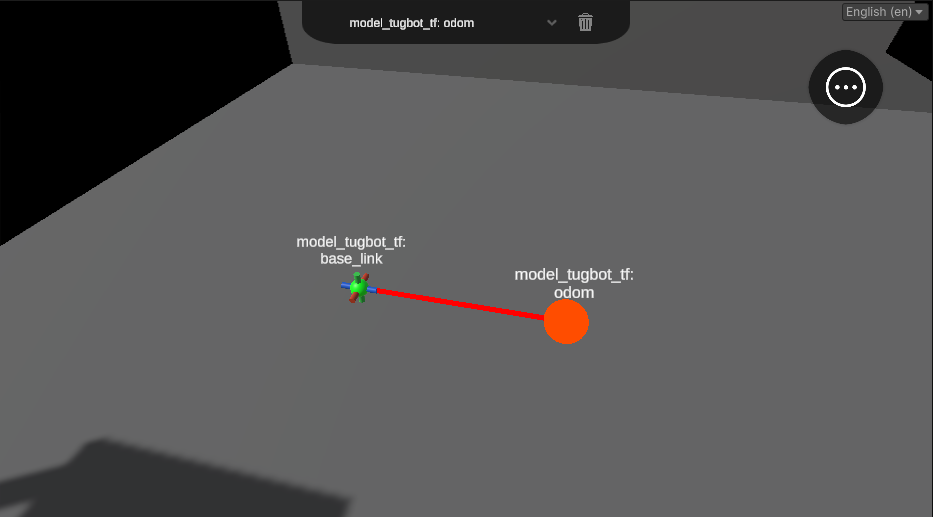
\includegraphics[width=0.8\textwidth]{imagenes/capturas_app/tf.png}
    \caption{Visualización \textit{transforms}}
    \label{fig:transforms_visualization}
\end{figure}

En la Figura \ref{fig:lineal_speed_visualization} se puede observar cómo se muestra en la aplicación la velocidad lineal. Esta variable es 
visualizada empleando un vector de color azul en el que la longitud indica la dirección del desplazamiento, de manera que cuanto mayor sea el vector, 
a mayor velocidad se desplazará el \textit{frame}. Además, en la parte posterior del movimiento se puede observar otro elemento que indica el \textit{trail}, es decir,
la trayectoria seguida por el \textit{frame}.
\begin{figure}[htbp]
    \centering
    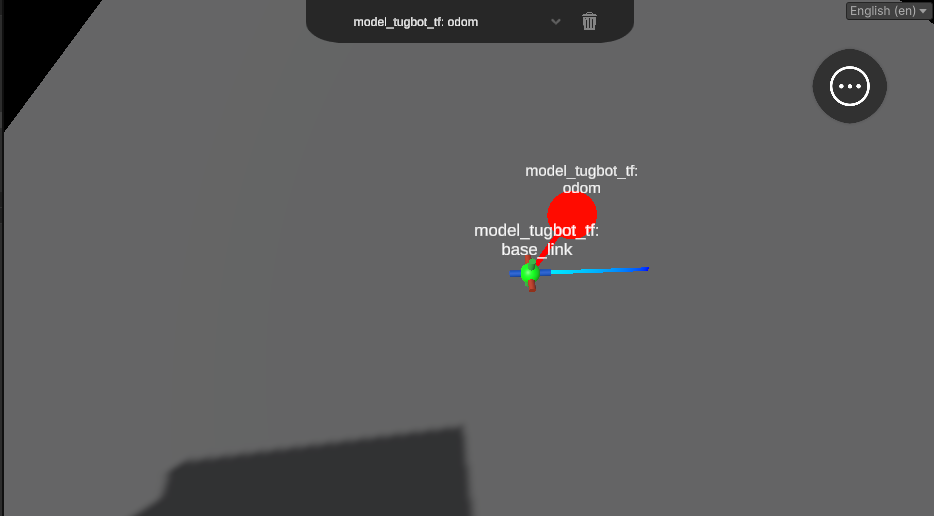
\includegraphics[width=0.8\textwidth]{imagenes/capturas_app/speed.png}
    \caption{Visualización velocidad lineal}
    \label{fig:lineal_speed_visualization}
\end{figure}

En la Figura \ref{fig:angular_speed_visualization} se puede observar cómo se muestra en la aplicación la velocidad angular. Esta variable 
es visualizada mediante un elemento toroidal que indica el eje en el que se está realizando el giro; el color, a su vez, indica que la velocidad 
se encuentra dentro de ciertos márgenes (verde para velocidades menores a 0,5 rad/s, amarillo para velocidades entre 0,5 rad/s y 1 rad/s).
\begin{figure}[htbp]
    \centering
    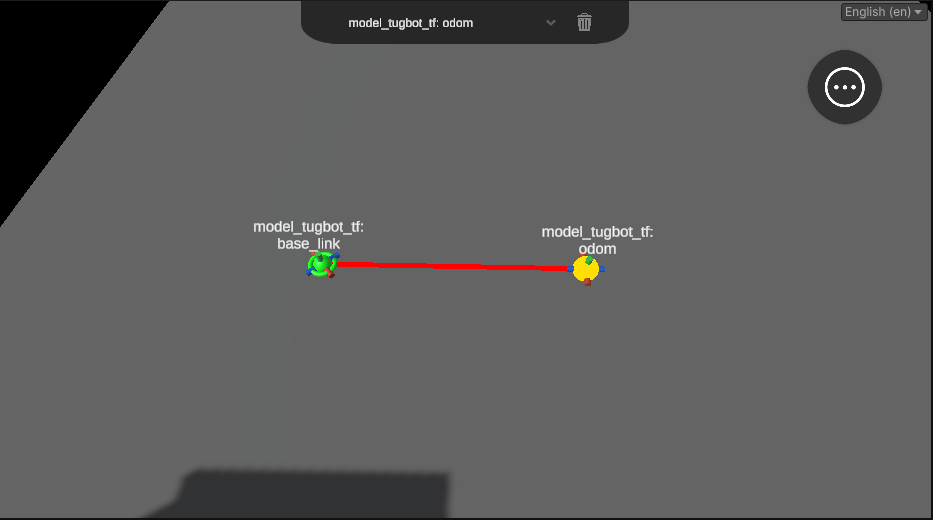
\includegraphics[width=0.8\textwidth]{imagenes/capturas_app/angular_speed.png}
    \caption{Visualización velocidad angular}
    \label{fig:angular_speed_visualization}
\end{figure}

Las Figuras \ref{fig:frame_occultation} y \ref{fig:frame_visualization} muestra la funcionalidad de visualización y ocultación de \textit{frames}. 
La aplicación proporcionará la lista de \textit{frames} y el 
usuario seleccionará aquellos que desee ocultar/mostrar 
\begin{figure}[htbp]
    \centering
    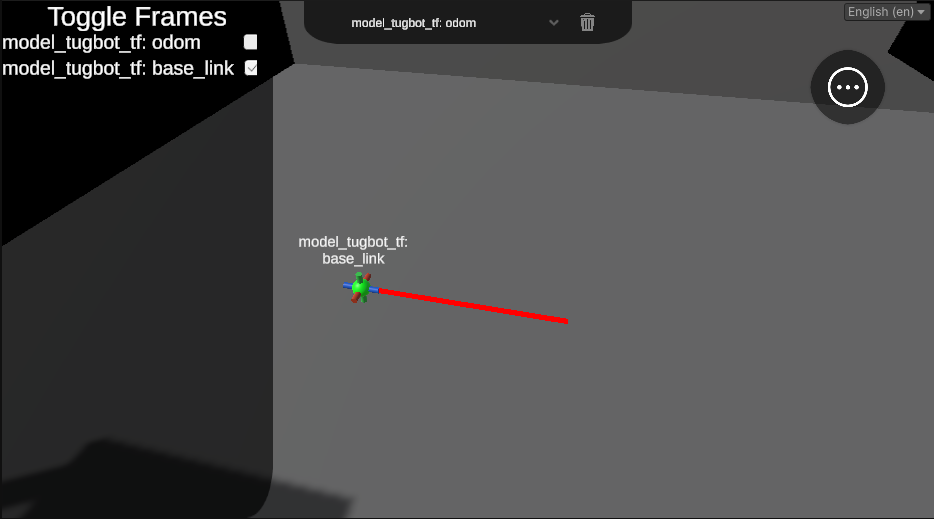
\includegraphics[width=0.8\textwidth]{imagenes/capturas_app/toggle_frames_2.png}
    \caption{Ocultación de frames}
    \label{fig:frame_occultation}
\end{figure}
\begin{figure}[htbp]
    \centering
    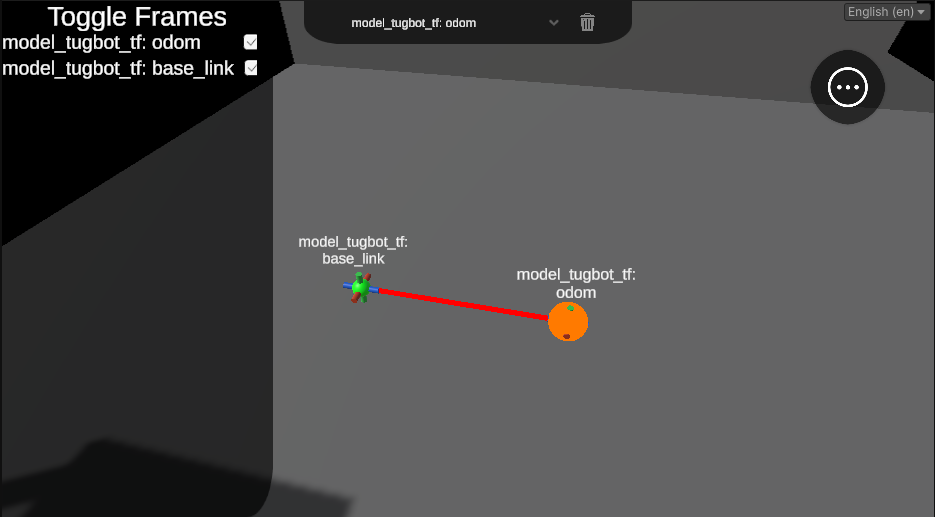
\includegraphics[width=0.8\textwidth]{imagenes/capturas_app/toggle_frames_1.png}
    \caption{Visualización de frames}
    \label{fig:frame_visualization}
\end{figure}

La Figura \ref{fig:teleop} muestra la funcionalidad de teleoperación de robots. El usuario deberá seleccionar el \textit{topic} objetivo
de la comunicación y mediante el accionamiento del \textit{joystick} virtual o los botones enviará mensajes de movimiento.
La aplicación permite, además, modificar parámetros de la velocidad lineal, vertical y angular.
\begin{figure}[htbp]
    \centering
    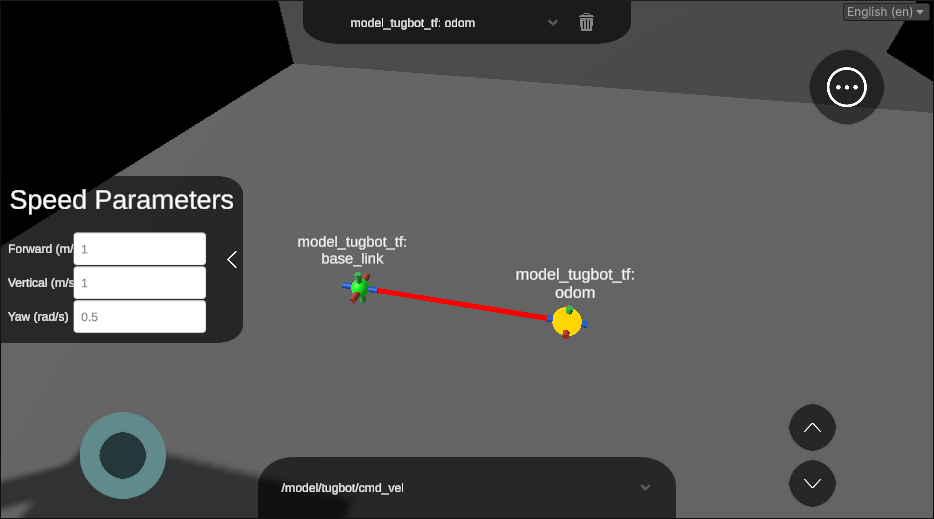
\includegraphics[width=0.8\textwidth]{imagenes/capturas_app/teleop.png}
    \caption{Teleoperación}
    \label{fig:teleop}
\end{figure}

Similar a la funcionalidad anterior es la planificación de rutas. La Figura \ref{fig:path_plan} muestra su interfaz. El usuario, de igual manera,
seleccionará el \textit{topic} objetivo de la comunicación y el \textit{frame} objetivo empleando los selectores inferiores y superiores respectivamente.
Posteriormente, seleccionará uno o varios puntos en el mundo en el que se siturán marcadores azules unidos por una línea indicando el recorrido a realizar.
Esta ruta no será ejecutada hasta que el usuario no envíe el mensaje mediante el botón con el avión de papel como icono. El botón de la izquierda eliminará uno a uno los 
marcadores, de modo que se puede rehacer la ruta a conveniencia. 
\begin{figure}[htbp]
    \centering
    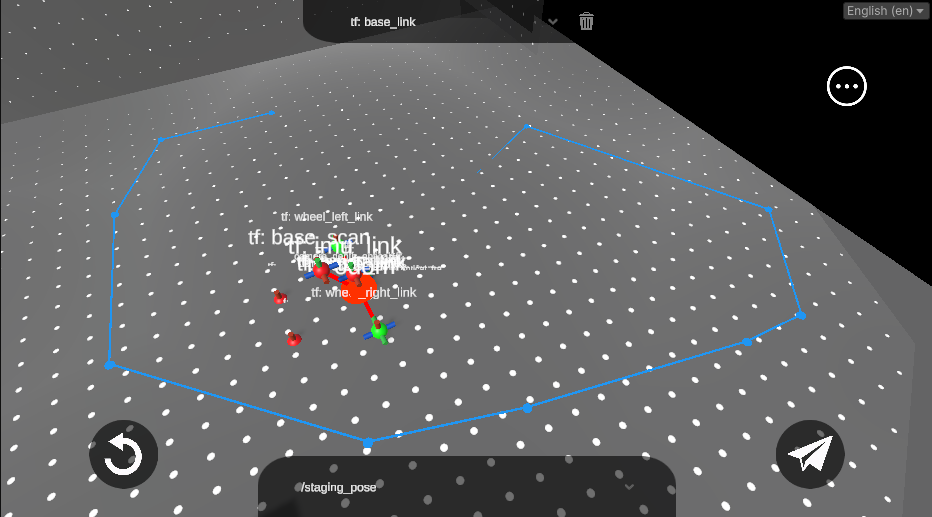
\includegraphics[width=0.8\textwidth]{imagenes/capturas_app/path_plan.png}
    \caption{Planificación de ruta}
    \label{fig:path_plan}
\end{figure}

La Figura \ref{fig:measure_frames} muestra la funcionalidad de medidas entre frames. El uisuario seleccionará dos \textit{frames}; estos cambiarán de color a 
azul parpadeante y se mostrará en la ventana izquieda diferentes parámetros como su distancia en metros y su rotación.
\begin{figure}[htbp]
    \centering
    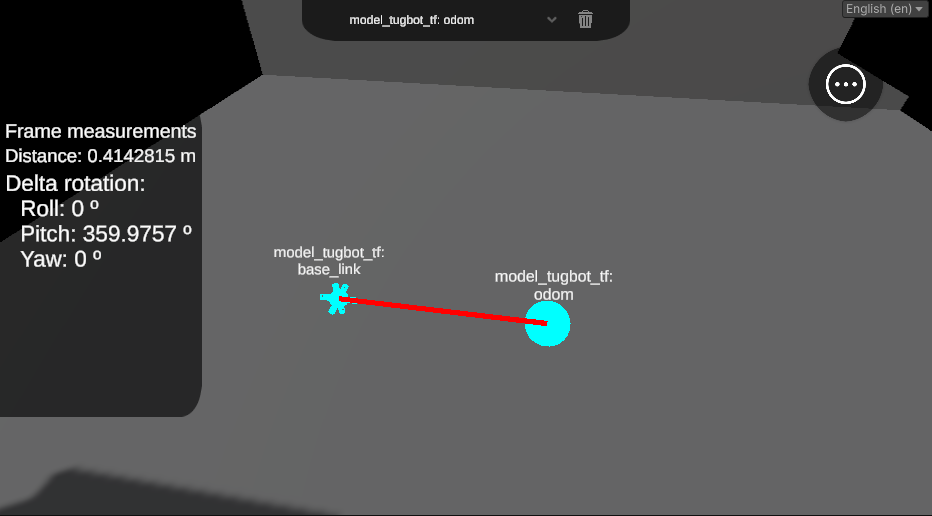
\includegraphics[width=0.8\textwidth]{imagenes/capturas_app/measure_frames.png}
    \caption{Medición de frames}
    \label{fig:measure_frames}
\end{figure}

La Figura \ref{fig:frame_scale_adjustment} muestra la funcionalidad de escalado de los \textit{frames} en la que el usuario seleccionará un \textit{frame} 
dejando el dedo unos instántes sobre la pantalla. El objeto cambiará entonces de color a modo transparente parpadeante y será entonces cuando el 
usuario mediante un pellizco en la pantalla podrá ampliar y reducir la escala del elemento.
\begin{figure}[htbp]
    \centering
    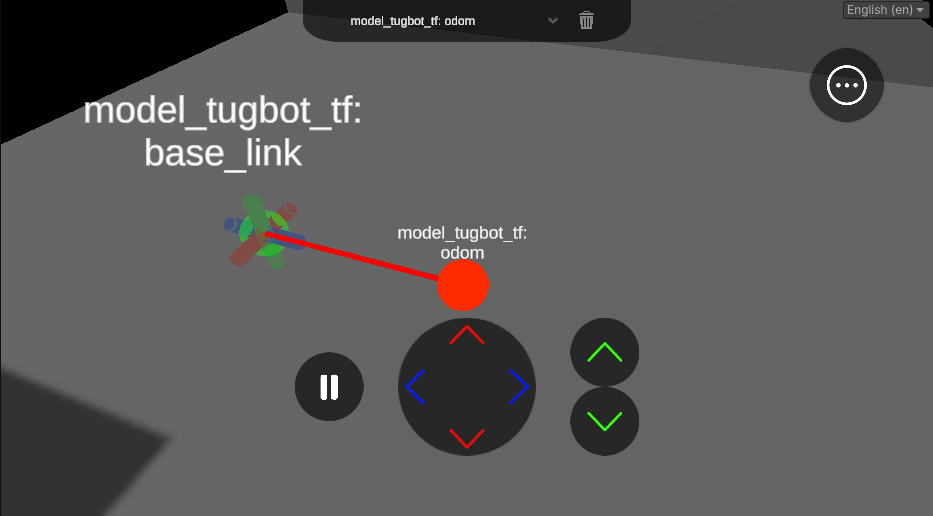
\includegraphics[width=0.8\textwidth]{imagenes/capturas_app/frame_adjustment_1.png}
    \caption{Ajuste de escala de frames}
    \label{fig:frame_scale_adjustment}
\end{figure}

Las Figuras \ref{fig:point_cloud_config} y \ref{fig:point_cloud_visualization} muestran la funcionalidad de la visualización de nube de puntos.
Inicialmente, el usuario debe configurar la asociación entre el \textit{frame} y el \textit{topic} de nube de puntos puesto que se trata de una relación 
que no puede presuponerse (como se indicó en el apartado de la implementación del sistema). Una vez realizada la asociación, la nube de puntos se visualizará en
el \textit{frame} correspondiente.
\begin{figure}[htbp]
    \centering
    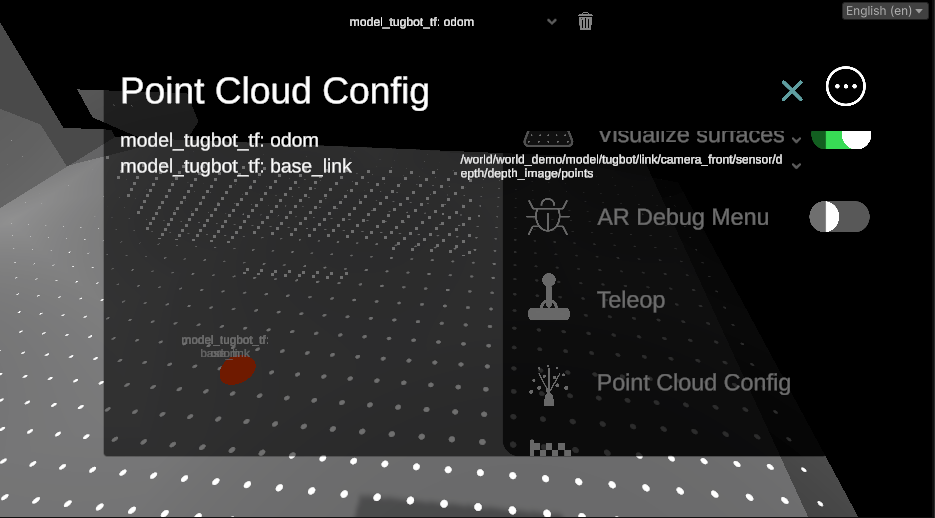
\includegraphics[width=0.8\textwidth]{imagenes/capturas_app/point_cloud_config.png}
    \caption{Configuración de nube de puntos}
    \label{fig:point_cloud_config}
\end{figure}
\begin{figure}[htbp]
    \centering
    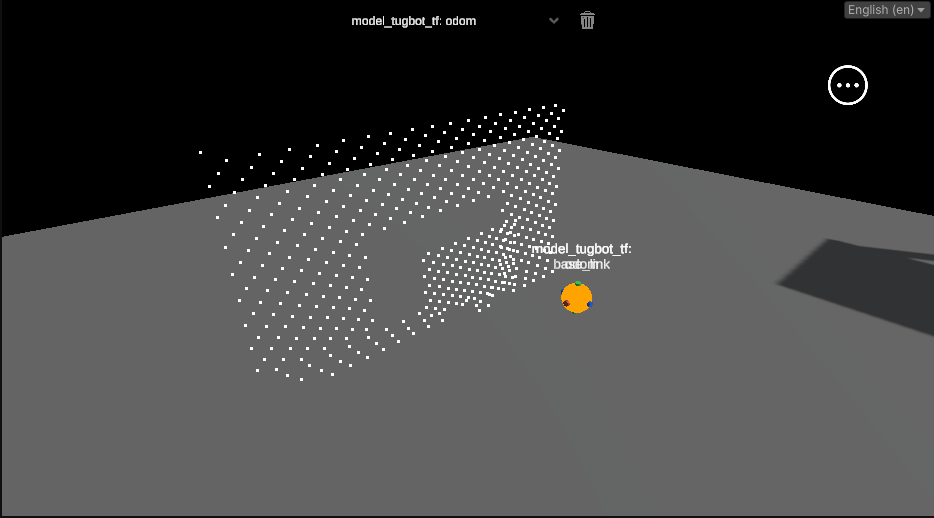
\includegraphics[width=0.8\textwidth]{imagenes/capturas_app/point_clouds.png}
    \caption{Visualización de nube de puntos}
    \label{fig:point_cloud_visualization}
\end{figure}

La Figura \ref{fig:topic_echo} muestra la funcionalidad de suscripción a tema para su visualización directa en la aplicación. El usuario
seleccionará un \textit{topic} y un tipo de mensaje de los selectores y pulsará en confirmar. Tras esto, los mensajes publicados en 
ese tema se visualizarán en la parte derecha de la pantalla. Para parar la visualización el usuario puede pulsar en "Parar" o "Stop".
\begin{figure}[htbp]
    \centering
    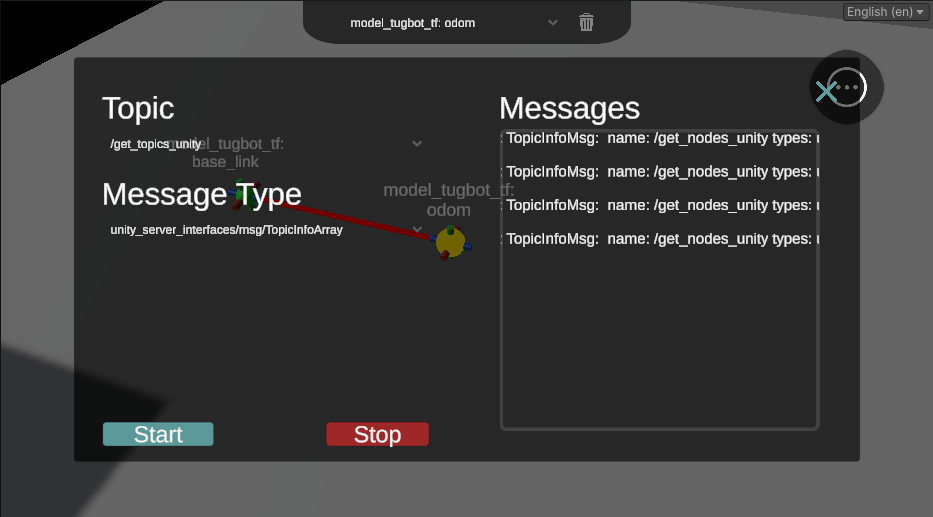
\includegraphics[width=0.8\textwidth]{imagenes/capturas_app/topic_echo.png}
    \caption{Suscripción a \textit{topics}}
    \label{fig:topic_echo}
\end{figure}

La Figura \ref{fig:topic_publish} muestra la funcionalidad de publicación en un tema. El usuario seleccionará un \textit{topic} de los
disponibles, un tipo de mensaje y cumplimentará el mensaje. Tras seleccionar la frecuencia de publicación en el tema confirmará la publicación y 
el mensaje será enviado siguiendo los parámetros correspondientes al \textit{topic} correspondiente.
\begin{figure}[htbp]
    \centering
    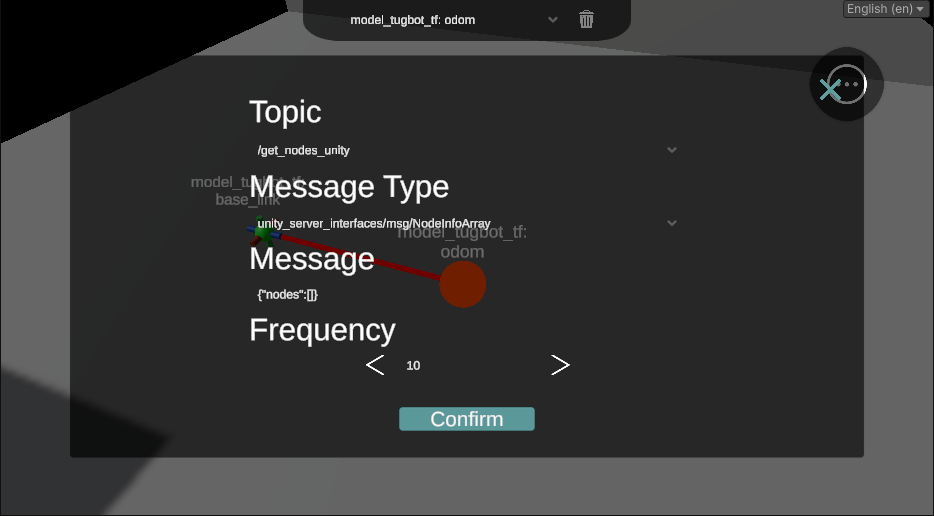
\includegraphics[width=0.8\textwidth]{imagenes/capturas_app/topic_publish.png}
    \caption{Publicación en \textit{topic}}
    \label{fig:topic_publish}
\end{figure}

La Figura \ref{fig:param_change} muestra la funcionalidad de configuración de parámetros de los nodos de ROS. El usuario seleccionará el nodo objetivo,
el parámetro que quiera modificar e introducirá el nuevo valor siguiendo la guía del valor anterior. Una vez cumplimentado los datos correspondientes, 
podrá enviar el nuevo valor pulsando "Enviar" o "Save".
\begin{figure}[htbp]
    \centering
    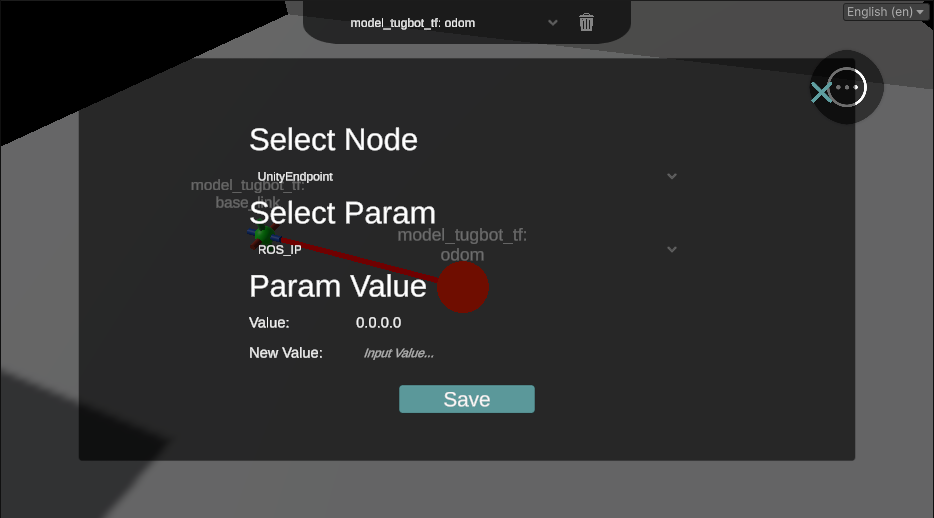
\includegraphics[width=0.8\textwidth]{imagenes/capturas_app/param_change.png}
    \caption{Configuración de parámetros}
    \label{fig:param_change}
\end{figure}

La Figura \ref{fig:app_config} muestra la interfaz de configuración de la aplicación. En esta se podrá modificar el idioma de la aplicación, el estándar \textit{AprilTag}
a emplear en la aplicación y parámetros de la conexión al servidor ROS como la dirección IP o el puerto entre otros.
\begin{figure}[htbp]
    \centering
    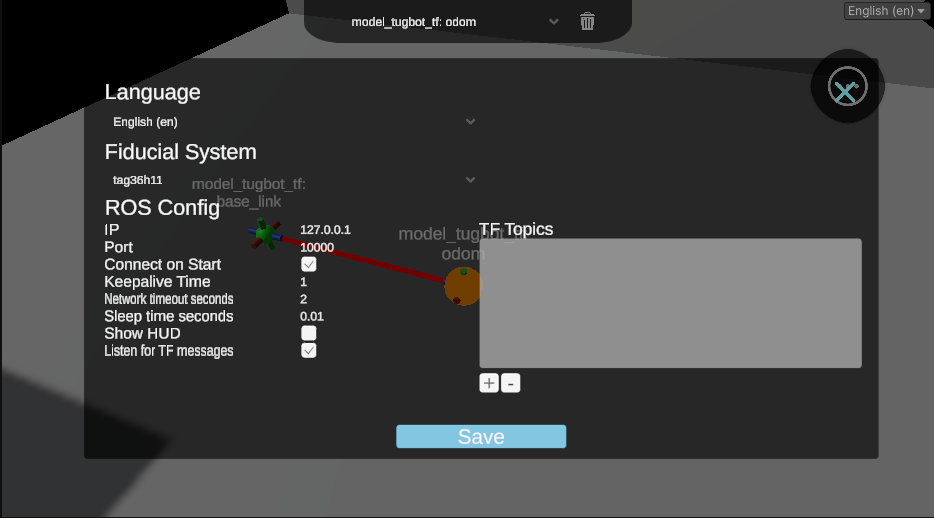
\includegraphics[width=0.8\textwidth]{imagenes/capturas_app/config.png}
    \caption{Configuración}
    \label{fig:app_config}
\end{figure}

\section{Validación de los requisitos}
A continuación se muestra el resumen de los requisitos funcionales y no funcionales con su respectivo estado.
\begin{longtable}{|p{4cm}|p{4cm}|}
\hline
\textbf{Requisito} & \textbf{Estado} \\
\hline
RF-001 & Cumplido \\
\hline
RF-002 & Cumplido \\
\hline
RF-003 & Cumplido \\
\hline
RF-004 & Cumplido \\
\hline
RF-005 & Cumplido \\
\hline
RF-006 & Cumplido \\
\hline
RF-007 & Cumplido \\
\hline
RF-008 & Cumplido \\
\hline
RF-009 & Cumplido \\
\hline
RF-010 & Cumplido \\
\hline
RF-011 & Cumplido \\
\hline
RF-012 & Cumplido \\
\hline
RF-013 & Cumplido \\
\hline
RF-014 & Cumplido \\
\hline
RF-015 & Cumplido \\
\hline
RF-016 & Cumplido \\
\hline
RF-017 & Cumplido \\
\hline
RF-018 & Cumplido \\
\hline
RF-019 & Cumplido \\
\hline
RF-020 & Cumplido \\
\hline
RF-021 & Cumplido \\
\hline
RF-022 & Cumplido \\
\hline
RF-023 & Cumplido \\
\hline
RF-024 & Cumplido \\
\hline
RF-025 & Cumplido \\
\hline
RF-026 & Cumplido \\
\hline
RF-027 & Cumplido \\
\hline
\hline
RNF-001 & NA \\
\hline
RNF-002 & NA \\
\hline
\caption{Estado de los requisitos funcionales y no funcionales}
\end{longtable}

Como se puede observar, todos los requisitos funcionales han sido cumplimentados en el desarrollo de la aplicación. Por otro lado, los no funcionales no 
pueden evaluarse de la misma forma que su contraparte funcional, puesto que no se trata de si se ha introducido una funcionalidad concreta o no, sino 
de la medida en la que se encuentran cubiertos en la aplicación, así pues, no puede darse una respuesta en firme sin que los usuarios finales juzguen con su criterio
la aceptación de esos requisitos.

\section{Resultados de las pruebas}
En esta sección se mostrarán la cantidad de pruebas diferentes realizadas, las que han sido un éxito y las que no han sido superadas 
\footnote{Solo se incluyen las realizadas en la etapa de pruebas. Las llevadas a cabo en la etapa de desarrollo no se computan. }.
\begin{longtable}{|p{4cm}|p{4cm}|p{4cm}|p{4cm}|}
\hline
\textbf{Prueba} & \textbf{Pruebas Realizadas} & \textbf{Pruebas Superadas} & \textbf{Pruebas No Superadas} \\
\hline
CP-01 & - & - & - \\
\hline
CP-02 & 10 & 10 & 0 \\
\hline
CP-03 & 6 & 6 & 0 \\
\hline
CP-04 & - & - & - \\
\hline
CP-05 & 1 & 1 & 0 \\
\hline
CP-06 & 1 & 1 & 0 \\
\hline
CP-07 & 1 & 1 & 0 \\
\hline
CP-08 & 3 & 3 & 0 \\
\hline
CP-09 & 1 & 1 & 0 \\
\hline
CP-10 & 1 & 1 & 0 \\
\hline
CP-11 & 1 & 1 & 0 \\
\hline
CP-12 & 1 & 1 & 0 \\
\hline
CP-13 & 1 & 1 & 0 \\
\hline
CP-14 & 1 & 1 & 0 \\
\hline
CP-15 & 1 & 1 & 0 \\
\hline
CP-16 & 1 & 1 & 0 \\
\hline
CP-17 & 1 & 1 & 0 \\
\hline
CP-18 & 1 & 1 & 0 \\
\hline
CP-19 & 1 & 1 & 0 \\
\hline
CP-20 & 1 & 1 & 0 \\
\hline
CP-21 & 5 & 5 & 0 \\
\hline
CP-22 & 5 & 5 & 0 \\
\hline
CP-23 & 3 & 3 & 0 \\
\hline
CP-24 & 5 & 5 & 0 \\
\hline
CP-25 & 5 & 5 & 0 \\
\hline
CP-26 & 5 & 5 & 0 \\
\hline
CP-27 & 5 & 5 & 0 \\
\hline
CP-28 & 5 & 5 & 0 \\
\hline
CP-29 & 5 & 5 & 0 \\
\hline
CP-30 & 3 & 3 & 0 \\
\hline
CP-31 & 4 & 4 & 0 \\
\hline
CP-32 & 4 & 4 & 0 \\
\hline
CP-33 & 5 & 5 & 0 \\
\hline
CP-34 & 3 & 3 & 0 \\
\hline
CP-35 & 2 & 2 & 0 \\
\hline
CP-36 & 8 & 8 & 0 \\
\hline
\caption{Resultados de las pruebas de integración}
\end{longtable}

% \section{Rendimiento}
% % Si aplica: tiempo de respuesta, consumo de memoria, tasa de errores, escalabilidad, capacidad de procesamiento, etc.

\section{Limitaciones encontradas}
Durante el desarrollo del proyecto se experimentó con la compilación cruzada del \textit{framework} de ROS para Android, 
de manera que se pudiera incluir como un \textit{plugin} dentro de la aplicación Unity, sin embargo, la dependencia
\textit{rmw\_implementation} no es posible compilarla en esta plataforma en el tiempo del desarrollo de la aplicación,
ya que necesita de unas modificaciones excesivas en la librería base, que no entran dentro del alcance propuesto en el proyecto.

Para paliar estas restricciones temporales, se optó por investigar la posibilidad de la compilación cruzada de \textbf{micro-ROS}
igualmente para Android. La compilación y ejecución de este marco de trabajo fue un éxito, sin embargo, durante un análisis 
y experimentación más exhaustivo, se encontró que no mantiene el grafo ROS necesario para el correcto funcionamiento de la aplicación
(visualización de diferentes elementos)
por lo que se continuó con la estrategia provisional que había sido introducida en los primeros incrementos del proyecto, 
haciendo necesaria una dependencia externa (\textit{ROS-TCP-Connector} y nodo propio con capacidad de mantener el grafo ROS) 
que actúe como soporte para la aplicación y aligerando, por otra parte, los recursos necesarios en el dispositivo móvil.

Como sustituto a \textbf{micro-ROS}, se investigó la posibilidad de instalar en un dispositivo Android una 
máquina virtual ligera Ubuntu empleando \textit{Termux}. A pesar de los problemas iniciales de versionado de Ubuntu, la 
instalación en el terminal fue un éxito, pudiendo ejecutar una instancia ROS en el \textit{smartphone}. De esta manera, 
se abre una línea nueva en la que el móvil ejecute tanto ROS como la aplicación de realidad aumentada, desechando la necesidad
de dispositivos externos.

Por otro lado, en la funcionalidad de la visualización de nube de puntos, debido a la cantidad de datos procedentes de los sensores 
que han de procesarse se observa una caida repentinas de \textit{frames} de la aplicación. Para paliar estos efectos, se ha realizado
un muestreo de los valores proporcionados reduciendo los elementos que deben ser dibujados; además, se ha optado por emplear dos \textit{buffers} de 
datos, uno para la lectura y otro para la escritura y actualizar la malla visualizada cada 15 \textit{frames} de la aplicación. 
Aún con todos estas técnicas, debido a que el redibujado de las mallas de puntos es costosa a nivel computacional y que puesto a que la aplicación está 
destinada a dispositivos móviles y no se pueden emplear elementos de computación paralela como las tarjetas de vídeo, la problemática es todavía presente.

\section{Resumen de resultados}
La aplicación desarrollada cumple con todos los requisitos funcionales propuestos en el proyecto, sin embargo, los no funcionales no pueden ser evaluados de la misma manera,
puesto que no se trata de si se ha introducido una funcionalidad concreta o no, sino de la medida en la que se encuentran cubiertos en la aplicación, así pues, no puede darse
una respuesta en firme sin que los usuarios finales juzguen con su criterio la aceptación de estos.

Por otro lado, se han encontrado limitaciones en la aplicación que no han podido ser resueltas en el tiempo de desarrollo del proyecto, 
como la imposibilidad de compilar ROS para Android y la problemática de la visualización de nubes de puntos. 
A pesar de esto, se ha conseguido desarrollar una aplicación funcional que permite la visualización y control de robots mediante realidad aumentada.

